\documentclass[12pt,oneside]{book}
\pagestyle{headings}

% Note that the line below could be modified to suit a
% particular system since the "geometry" package behaves
% differently in Unix, Windows and Mac, especially for the
% top margins.
% Adjust the parameter "top" (measuring the height of the
% space allocated to a header) and "headsep" (measuring
% the distance from the bottom of the header to the
% first line of text.
\usepackage[top=1.3in,left=1.5in,bottom=1in,right=1in,headsep=0.5in]{geometry}

\usepackage{setspace}
\onehalfspacing
%\doublespacing

% Headers and footers for thesis
\usepackage{fancyhdr}

\markboth{}{}
\newcommand\startchapter[1]{\chapter{#1}\thispagestyle{myheadings}}
\newcommand\startappendix[1]{\chapter{#1}\thispagestyle{myheadings}}
\newcommand\startfirstchapter[1]{\chapter{#1}}

% Manual addition of section to Table of Contents
\newcommand\TOCadd[1]{\newpage\phantomsection\addcontentsline{toc}{chapter}{#1}}

% Float Customization
\renewcommand{\floatpagefraction}{0.01}

% Customization of Tables of Contents and List of Figures/Tables
\usepackage{tocloft}
\renewcommand\cfttabpresnum{Table\ }
\renewcommand\cfttabnumwidth{0.75in}
\renewcommand\cftfigpresnum{Figure\ }
\renewcommand\cftfignumwidth{0.80in}
\newcommand{\HRule}{\rule{\linewidth}{0.5mm}}


% Long Table and decimal aligned columns
\usepackage{dcolumn}
\usepackage{longtable}
\usepackage{multicol}
\usepackage{multirow}

% Mathematics support
\usepackage{amsmath}
\usepackage{amsthm}
\usepackage{amssymb}


% Text Control
\usepackage{xspace}
\usepackage{textcase}

% Graphics
\usepackage{wasysym}
\usepackage{graphics}
\usepackage{graphicx}   % A package to allow insertion of
                        % external image files

\usepackage{float}

\usepackage{placeins}
\usepackage{longtable} % <---- new
\usepackage{fancyhdr,graphicx,amsmath,amssymb}
\usepackage{fullpage}
\usepackage{times}
\usepackage{float}
\usepackage{xr}
\usepackage{caption}
\usepackage{xcolor}
\usepackage[linesnumbered,ruled,vlined]{algorithm2e}
\SetKwRepeat{Struct}{struct \{}{\}}%
\SetKwRepeat{Union}{union \{}{\}}%
\newcommand\mycommfont[1]{\footnotesize\ttfamily\textcolor{blue}{#1}}
\SetCommentSty{mycommfont}
\usepackage{listings}
 \lstset{
 basicstyle=\ttfamily\scriptsize,
 columns=fullflexible,
 frame=single,
 breaklines=true,
 postbreak=\mbox{\textcolor{red}{$\hookrightarrow$}\space},
 }
 \usepackage[flushleft]{threeparttable}
 \usepackage[titletoc]{appendix}
\usepackage{placeins}
\usepackage{longtable} % <---- new

\usepackage{caption}
\begin{document}

% Front Matter
\input frontmatter/fm

\newpage

	\startfirstchapter{Introduction}
\label{chapter:introduction}
Vulnerabilities in software enable the exploitation of the computer or system they are running on. Therefore, the emphasis placed on computer security particularly in the field of software vulnerabilities has increased dramatically. It's important for software developers to build secure applications. Unfortunately, building secure software is expensive. The vendors usually comply with their own quality assurance measures which focus on marketable concerns while leaving security to a lower priority or even worse, totally ignore it. Therefore, fully relying on the vendor of the software to secure your system and data is unpractical and risky.\cite{dowd_art_2006}

Software security review conducted by a third party is neccessary. One approach of software security review is software auditing. It is a process of analyzing the software in forms of source code or binary. This auditing can uncover some hard to reveal vulnerabilities which might be exploited by hackers. Identification of these security holes can save the users of the software from putting their sensitive data and business resources at risk.\cite{dowd_art_2006}

Most of the software vulnerabilities are stimulated by malicious data. So it is valuable to understand how this malicious data triggers the unexpected behaviors of the system. In most cases, this malicious data is injected by attackers into the system to trigger the exploitation. In some complex systems, several programs work together to provide service or functionality. In these situations, the malicious data might have passed through multiple components of the system and be modified before it reaches the vulnerable point and ultimately triggers an exploitable condition of the system. As a consequence, the flow of data throughout the system's different programs is considered to be one of the most important aspects to analyze during the security review.\cite{dowd_art_2006}

The data flow among various programs within a system or across different systems helps to understand how the system works as well as potentially disclose the vulnerabilities in a system. There are multiple mechanism to grab the data across programs. And the methods for obtaining this data flow can affect the analysis results greatly. 

In this research, I developed a method to identify communications between programs by analysing the assembly level execution traces. This method can guide the security engineers to investigate the communications of the programs in the circumstance that they have the captured execution traces and want to understand the interaction behaviour of the programs. The research is not specific for vulnerabilities detection but generalized for the comprehension of the interacting behaviour of two programs.

\section{Motivation}
This project started with an informal requirement from DRDC for visualizing multiple assembly traces to assist their software and security analysis. The literature review and the conversation with DRDC help to clarify the goal and decide the target of this research. In this section, I discuss the need of performing assembly trace investigation for communication analysis. First I explain why the security engineers perform assembly trace analysis. Then I elaborate why they need to perform communication analysis at assembly trace level. 

\subsection{Why Assembly Trace Analysis}
Dynamic analysis of program is adopted mainly in software maintenance and security auditing\cite{zhang2010detecting}, \cite{cai2016sworddta}, \cite{somorovsky2016systematic}. Sanjay Bhansali et al. claimed that program execution traces with the most intimate detail of a program's dynamic behavior can facilitate the program optimization and failure diagnosis. Jonas Tr{\"u}mper et al. give a example of how tracing can facilitate software-maintenance tasks \cite{trumper2012maintenance}.

The dynamic analysis can be done using debuggers, however, debuggers would halt the execution of the system and result in a distortion of the timing behavior of the running system \cite{trumper2012maintenance}. Instead, tracing a running program with instrumentation would provide more accurate run time behaviour information about the system. 

The instrumentation of the tracing can be done at various levels of granularity, such as programming language or machine language instructions. The access to a software can be divided into five categories, with variations: source only, binary only, both source and binary access, checked build, strict black box. Only having the binary is common when performing vulnerability research on closed-source commercial software\cite{dowd_art_2006}. In this case, assembly level tracing is the only option to do a security review of the software.

Since the binary code is what is running on the system, binary tracing is more representative of actual situation than the source code.  Some bugs might appear because of a compilation problem or because the compiler optimized away some code that was
necessary to make the system secure. The piece of code listed below is an example in which the line of code resetting the password before the program end would be optimized away by the compliers if they implement the dead store elimination\cite{howard2003writing}. For example, with the -fdse option, the GNU Compiler Collection(GCC) will perform the dead store elimination and -fdse is enabled by default at -O and higher \cite{gcc}. This made the user's password stayed in memory, which is considered as potential security risk. However, looking at the source code does not reveal the problem.

\begin{lstlisting}[language=C++, caption= Password Fetching Example ]
#include <iostream>
#include <string>
#include <conio.h>
using namespace std;
int main(){
   string password ="";
   char ch;
   cout << "Enter password";
   ch = _getch();
   while(ch != 13){//character 13 is enter
      password.push_back(ch);
      cout << '*';
      ch = _getch();
   }   
   if(checkPass(password)){
     allowLogin();
   }  
   password ="";
}
\end{lstlisting}

\subsection{Why Communication Analysis with Assembly Traces}
Programs nowadays do not always work isolated. The communication and interaction between modules affect the behaviour of the software. Without knowing how a program works with others, an analysis of the isolated execution trace on a single computer is usually futile. Data flow tracing between programs is essential to review both the design and implementation of the software.

Many network sniffer, such as Wireshark\cite{_wireshark_????} and Tcpdump\cite{tcpdump_tcpdump/libpcap_????}, can help to capture the data flow across the network. However, this method  is insufficient because security problems can occur even if the information sent is correct. Therefore, analysing the communications with transmitted data in instruction and memory access level is a solid way to evaluation the security of a system.

Shameng Wen et al. argued that fuzz testing and symbolic execution are widely applied to detect vulnerabilities in network protocol implementations. Their work focuses on designing a model which guides the symbolic execution for the fuzz testing \cite{wen2017model} but ignoring the analysis of the output, which is the execution traces. Further more, their work focuses only on the network protocol implementation and is not generalized to all communications.

Besides vulnerabilities detection and security analysis, communication analysis with assembly traces can also be a way to learn how the work is performed by the system or validate a specification of it. Our research partner DRDC provided some use cases in which they require the assistance of communication analysis to understand their systems. The first one is related to their work with embedded systems. These systems often have more than one processor, each specialized for a specific task, that coordinate to complete the overall job of that device.  In the other case, the embedded device will work with a normal computer and exchange information with it through some means
(USB, wireless, etc.).  For instance, the data might be coming in from an external sensor in an analog form, transformed by a Digital Signal Processor (DSP) in a device, sent to a more generic processor inside that device to integrate with other data then send wireless to an external computer. Being able to visualize more than one trace would help them follow the flow of data through the system at the same time that they trace the execution of the programs.

\section{Research Goal}
The goal of this research is to design a method for communication analysis using the execution traces of the interacting programs. This method should be general enough for all message based communication analysis between programs regardless of their programming language, host operating system or selected execution tracer. 

\section{Research Process}
Figure \ref{methodology} shows the overview of my research process with three abstracted stages. However, The approach of this research is not a forthright process. Instead, it is a back and forth one, for example the implementation changed several times with the changes of the model, and the models was modified based on the understanding throughout the implementation. 

\begin{figure}[H]
  \centerline{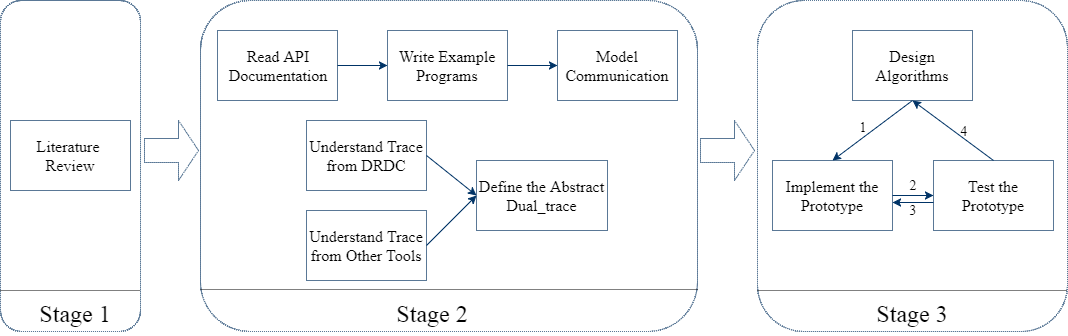
\includegraphics[scale=0.45]{Figures/methodology}}
  \caption{Research Approach overview}
  \label{methodology}
  \end{figure}

This research requires background knowledge of software security and vulnerabilities. I acquired the background knowledge basically from literature review. It helped me grab the essential concepts of software vulnerabilities and their categories, understand some facilities for vulnerabilities detection and software maintenance in the perspective of security. After that, I was convinced that communication analysis in assembly trace level would benefit software security engineers to understand the behaviour of software and detect software vulnerabilities. 

In order to analyze the communication of programs, I had to know how the communication works. For this purpose, I started the investigation by writing example simple programs with the Windows API and run them locally in my desktop. By understanding their behaviour and reading the Windows API documentation, I abstracted the communication model which is not operating system specific.

The abstract assembly trace definition was build on the generalization of the trace format provided by our research partner, DRDC. I don't have the access to their home-made assembly tracer which is based on PIN\cite{_pin_????}. Fortunately, they provideed me with a comprehensive document about the format of the captured trace and example traces. With these, I grasped the constructive view of the assembly execution trace. Further more, some other tools can also capture the required information in assembly level for communication analysis. This supports the generalization of the trace definition and the abstraction of the dual\_trace.

The implementation of the prototype and the communication analysis algorithms were developed in parallel. The high level communication identification algorithm and the specific algorithms for named pipe communication methods were abstracted based on the implementation, while the others are developed theoretically. Two experiments are designed to test this analysis method, the prototype and some algorithms. 


\section{Contributions}
The main contributions of these work can be summarized as:
\begin{itemize}
  \item \textbf{Communication Model:} The communication model in this thesis is an abstract model of the communications between two programs. It was abstracted from the understanding of several communication methods and is general for other communication methods that are not mentioned in this thesis.
  \item \textbf{Dual\_trace Formalization:} By understanding the assembly level execution traces, a dual\_trace was formalized to describe the information that needed for communication analysis. This model doesn't specify the format of the execution traces but defines what information is necessary to be contained to fulfil the analysis requirement. All execution traces that comply with this definition can be used for the analysis.
  \item \textbf{Communication Analysis Approach:} The overall approach to identify the communications in the dual\_trace is designed. Some algorithms were developed for the steps in this
approach regarding some communication methods or communication types.
  \item \textbf{Prototype:} A prototype is designed and implemented on Atlantis. This prototype demonstrate that the communication analysis approach is feasible. It is a unique tool for the security engineers to analyze the communications of programs via assembly execution trace analysis.
\end{itemize}

\section{Thesis Organization}
In Chapter 2, I summarize the related background information and knowledge needed to understand or related to this work including security and vulnerability, program communication mechanisms, program execution trace tools, and Atlantis. 

Chapter 3 describes the model of the communication between two programs. This model defines the communication in the context of trace analysis and discusses the properties of the communications. 

In Chapter 4, I first present the abstract dual\_trace formulation. Based on this formulation, I describe the communication analysis process and the essential algorithms.

In chapter 5, I present the implementation of a dual\_trace communication analysis prototype. 

In chapter 6, I present two experiments of communication analysis with dual\_traces using the implemented prototype. Notably, the result shows the communications are correctly identified. 

Finally, In chapter 7, I conclude the result of this research and outline the possible future work.
	\startchapter{Methodology}
The Methodology used for this work composed of 7 major steps. To make this work executable, 1)I defined the problem by understanding the requirement from our research partner DRDC. 2) I obtained the related background knowledge by literature review. Then 3) I model the abstract communication channels. Based on these channel models,4) I develop algorithms to synchronize the communication events happen in the channel. After that, 5) I match the real channels used in Windows Communication Foundation to my channel models, verify their consistency with my models. Finally 6)I implement the synchronization algorithms for the dual-trace analysis and verify them by the dual-traces from DRDC.


\label{chapter:problem}

\newlength{\savedunitlength}
\setlength{\unitlength}{2em}
\section{Define the Problem}
A dual-trace consists of two execution traces that are generated from two interacting applications. The trace analysis is based only on the assembly level execution trace which contain the instructions and memory change of a running application. Beside all the factors in single trace analysis, dual-trace analysis has to analyze the communications of the applications in the traces. A communication between two applications including the communication channel open, all data exchanging events, the communication channel close.  Correspondingly, a full communication definition in the dual-trace should consist of the channel opening events in both sides, data sending and receiving events, and the the channel closing events in both sides. Each of these events consist of function call and related data from the memory record. In some cases there might be some events lacking from the trace, such as no data exchange after a channel is open, or the traces end before the channel was closed. However, the channel open is critical, without that there is no way to locate all other events in the traces. The goal communication analysis of dual-trace is to rebuild all the user concerned communication channels from the dual-trace.


\section{Obtain Background Knowledge}
I did a some background reading in the reverse engineering filed, focusing more on the vulnerabilities detection domain to better understand the current state and needs. In addition, to locate the communication event of the dual-trace, I need to investigate the communication methods' APIs to understand their structure in the assembly level traces. I need to know how the functions for channel setup and the functions for messages sending/receiving work. The system functions I was looking for is in C++ level. I have to know the C++ function names, related parameters, return value and so on. Furthermore, to understand their structure in the assembly level trace, I have to know the calling conventions in assembly, such registers/memory for parameters or return value.

\section{Model the Communication Channels}
There are two abstract models for communication based on the communication behavior. One is the order guaranteed communication model and the other is order in-guaranteed communication model. I define  how the communication happens as well as all the data send/receive scenario in each model. Later on the real communication channels will be categorized into these two models. 


\section{Develop the Dual Trace Synchronization Algorithms}


\section{Apply the Channel Models to Windows APIs}
I investigate 4 types of communication channels in Windows Communication Foundation and match each of them to the developed channel model. These 4 types are Only Named pipe, MQMS, HTTP, and TCP/UDP socket. The matching includes two steps: 1. Put each type of communication channel in the modeling categories by verify the existence of the message send/receive scenario. 2. Define the function callings for each event types in the channel, such as channel opening and closing, data sending and receiving. 

\section{Implement the Trace Synchronization Algorithms}

\section{Evaluate the Communication Channel Rebuilt Feature in Atlantis}



\setlength{\unitlength}{\savedunitlength}

	\startchapter{Background}
\label{chapter:Bac}
In this section, I summarize the background knowledge or information that related to this work. First I generally describe software vulnerability. Second, I discuss the general definition of communication among programs and their categorization. Third, I introduce some tools for assembly level program debugging and analysis. Finally I introduce Atlantis, the existing assembly level execution trace analysis environment, on which the implementation of this work based.

\section{Software Vulnerability}
Software vulnerability detection is one of the use cases of the communication analysis with assembly level execution traces. The understanding of fundamentals of software vulnerability is necessary to comprehend some implicit concepts or design intention through out this thesis. 

Vulnerabilities, from the point of view of software security, are specific flaws or oversights in a program that can be exploited by attackers to do something maliciousexpose such as modify sensitive information, disrupt or destroy a system, or take control of a computer system or program. They are considered to be a subset of bugs. Input and Data Flow, interface and exceptional condition handling where vulnerabilities are most likely to surface in software and memory corruption is one of the most common vulnerabilities. The awareness of these two facts would make the security auditing and vulnerabilities detection have more clear focus. \cite{dowd_art_2006}

\section{Program Communications}
Programs can communicate with each other via diverse mechanisms. The communication happens among processes is known as inter-process communication. This refers to the mechanisms an operating system provides the process to share data with each other. It includes methods such as signal, socket, message queue, shared memory and so on.\cite{garrido2000inter} This communications can happen over network or inside a device. Based on their reliability, the communication methods can be simply divided into two categories: reliable communication and unreliable communication. In this work, communication methods belong to all both categories has been covered. However, I only discuss the message based communication methods while leave the control based communication, like remote function call for the future.

\section{Program Execution Tracing in Assembly Level}
The communication analysis discuss throughout this thesis is based on the assembly traces. Thurs capturing of the execution traces became a prerequisite of this work. DRDC has its own home-made tracer, the traces from which are used in the experiments of this research. However, the model and algorithms developed in this research is not limited with this specific home-made tracer. Any tracer that can capture sufficient information according to the model can serve this purpose.

There are many tools that can trace a running program in assembly instruction level.  IDA pro \cite{eagle_ida_2008} is a widely used tool in reverse engineering which can capture and analysis system level execution trace. Giving open plugin APIs, IDA pro allows plugin such as Codemap \cite{_c0demap/codemap:_????} to provide more sufficient features for "run-trace" visualization. PIN\cite{_pin_????} as a tool for instrumentation of programs, provides a rich API which allows users to implement their own tool for instruction trace and memory reference trace. Other tools like Dynamic \cite{brueningqz} and OllyDbg\cite{yuschuk2007ollydbg} also provide the debugging and tracing functionality in assembly level. 

\section{Atlantis}
Atlantis is a trace analysis environment developed in Chisel. It can support analysis for multi-gigabyte assembly traces. There are several features distinct it from all other existing tools and make it particularly successful in large scale trace analysis. These features are 1) reconstruction and navigation the memory state of a program at any point in a trace; b) reconstruction and navigation of system functions and processes; and c) a powerful search facility to query and navigate traces. The work of this thesis is not a extension of Atlantis. But it take advantages of Atlantis by reusing it existing functionality to assist the dual\_trace analysis.





    \externaldocument{../appendix/chapter_app}
\startchapter{Modeling}
\label{chapter:Mod}
In this chapter, I modeled the communication of two running programs. The modeling are based on the investigation of some common used communication methods. The communication methods are divided into two categories based on their data transmission properties. The terminology of using in this chapter can be found in \ref{term}.

\section{Communication Categorization and Communication Methods}
In general, there are two types of communication: reliable and unreliable in the terms of their reliability of data transmission. The reason to divide the communication methods into these two categories is that the data transmission properties of the communications fall in different categories affect the mechanism of the data verification in the identification algorithm. In the following two subsections, I summarize the characteristics of these two communication categories. The communication methods list in Table\ref{methodsInCategories} will be discussed further to provide more concrete comprehension. 
\begin{table}[H]
\centering
\caption{Communication Methods Discussed in This Work}
\label{methodsInCategories}
\begin{tabular}{|l|l|}
 \hline
\textbf{Reliable Communication}& \textbf{Unreliable Communication}\\
 \hline
Named Pipes & Message Queue   \\
TCP &  UDP \\
 \hline
\end{tabular}
\end{table}


\subsection{Reliable Communication}\label{reliable}
A reliable communication guarantees the data being sent by one endpoint of the channel is always received losslessly and in the same order in the other endpoint. For some communication methods, a channel can be closed before all sent data being received. With this property, the concatenated data in the receive stream of one endpoint should be the prefix of the concatenated data in the send stream of the other endpoint(potentially equal). Therefore, comparing the concatenated received data of one endpoint to the concatenated sent data of the other can verify the send and receive data.

\subsection{Unreliable Communication}\label{unreliable}
An unreliable communication does not guarantee the data being sent always arrive the receiver. Moreover, the data packets can arrive to the receiver in any order. However, the bright side of unreliable communication is that the packets being sent are always arrived as the origin packet, no data re-segmentation would happen. Accordingly, the send and receive data verification can be done by matching the data packet in a receive event to the data packet in a send event on the other side.

\subsection{Communication Methods}
In this section, I describe the mechanism and the basic data transfer characteristics of each communication method in Table\ref{methodsInCategories} briefly. Moreover, data transfer scenarios are represented correspondingly in diagrams for each communication method. 
 
\subsubsection{Named Pipe}
A named pipe provides FIFO communication mechanism for inter-process communication. It can be a one-way or a duplex pipe. \cite{khambattinamed}

The basic data transfer characteristics of Named Pipe are:
\begin{itemize}
  \item Bytes are received in order
  \item Bytes sent as a segment can be received in multiple segments(the opposite is not true)
  \item No data duplication
  \item If a sent segment is loss, all the following segments will lost(this happen when the receiver disconnect from the channel) 
  
\end{itemize}

Based on these characteristics, the data transfer scenarios of Named pipe can be exemplified in Figure\ref{namedpipe}. 
\begin{figure}[H]
\centerline{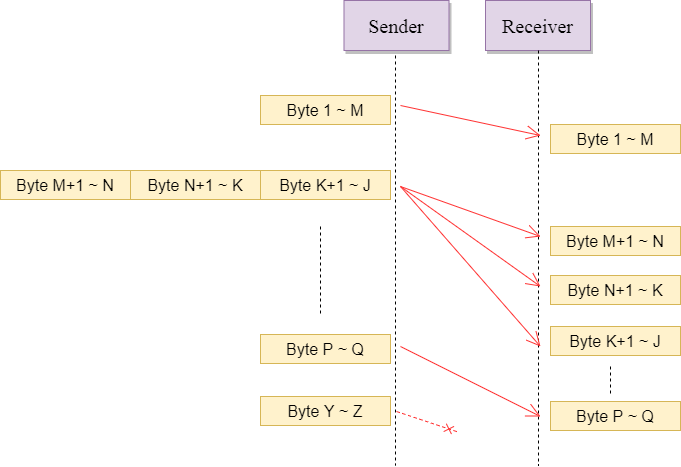
\includegraphics[scale=0.48]{Figures/namedpipe}}
\caption{Data Transfer Scenarios for Named Pipe}
\label{namedpipe}
\end{figure}

\subsubsection{Message Queue}
Message Queuing (MSMQ) is a communication method to allow applications which are running at different times across heterogeneous networks and systems that may be temporarily offline can still communicate with each other. Messages are sent to and read from queues by applications. Multiple sending applications can send messages to and multiple receiving applications can read messages from one queue.\cite{redkar2004pro} In this work, only one sending application versus one receiving application case is considered. Multiple senders to multiple receivers scenario can be divided into multiple sender and receiver situation. Both applications of a communication can send to and receive from the channel.

The basic data transfer characteristics of Message Queue are:
\begin{itemize}
  \item Bytes sent in packet and received in packet, no bytes re-segmented
  \item Packets can lost
  \item Packets received in order
  \item No data duplication
\end{itemize}
Based on these characteristics, the data transfer scenarios of Message Queue can be exemplified in Figure\ref{msmq}.
\begin{figure}[H]
\centerline{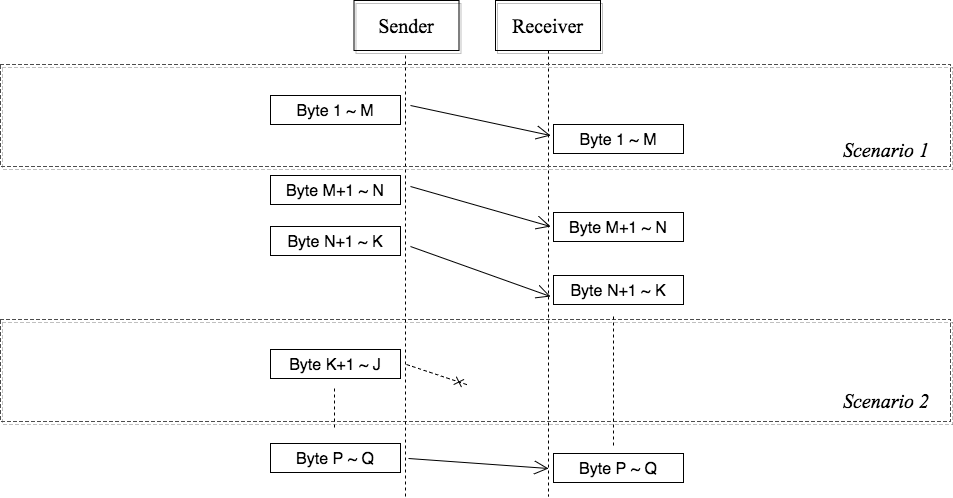
\includegraphics[scale=0.48]{Figures/msmq}}
\caption{Data Transfer Scenarios for Message Queue}
\label{msmq}
\end{figure}

\subsubsection{TCP}
TCP is the most fundamental reliable transport method in computer networking. TCP provides reliable, ordered, and error-checked delivery of a stream of octets between applications running on hosts in an IP network. The TCP header contains the sequence number of the sending octets and the acknowledge sequence this endpoint is expecting from the other endpoint(if ACK is set). The re-transmission mechanism is based on the ACK. 

The basic data transfer characteristics of TCP are:
\begin{itemize}
  \item Bytes received in order
  \item No data lost(lost data will be re-transmitted)
  \item No data duplication
  \item Sender window size is different from receiver's window size, so packets can be re-segmented
\end{itemize}

Based on these characteristics,  the data transfer scenarios of TCP can be exemplified in Figure\ref{tcp}.
\begin{figure}[H]
\centerline{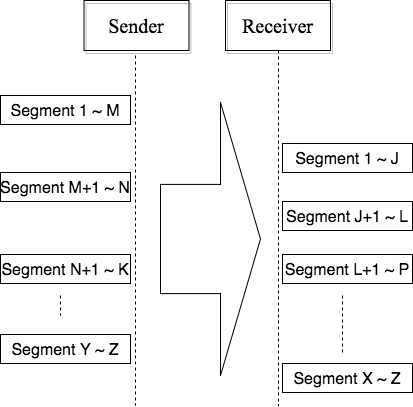
\includegraphics[scale=0.48]{Figures/tcp}}
 \caption{Data Transfer Scenarios for TCP}
\label{tcp}
\end{figure}

\subsubsection{UDP}
UDP is a widely used unreliable transmission method in computer networking. It is a simple protocol mechanism, which has no guarantee of delivery, ordering, or duplicate protection. This transmission method is suitable for many real time systems. 

The basic data transfer characteristics of UDP are:
\begin{itemize}
  \item Bytes sent in packet and received in packet, no re-segmentation
  \item Packets can lost
  \item Packets can be duplicated
  \item Packets can arrive receiver out of order
\end{itemize}

Based on these characteristics, the data transfer scenarios of UDP can be exemplified in Figure\ref{upd}.
\begin{figure}[H]
\centerline{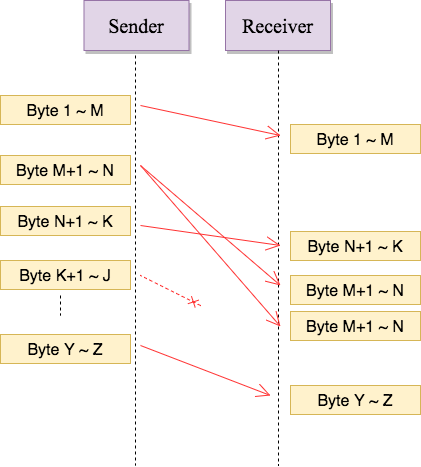
\includegraphics[scale=0.48]{Figures/udp}}
 \caption{Data Transfer Scenarios for UDP}
\label{upd}
\end{figure}

\section{Communication Model}\label{definition}
The communication of two programs is defined in this section. The communication in this work is data transfer activities between two running programs through a specific channel. Some collaborative activities between the programs such as remote procedure call is out of the scope of this research. Communication among multiple programs (more than two) is not discussed in this work. The channel can be reopened again to start new communications after being closed. However, the reopened channel will be treated as a new communication. The way that I define the communication is leading to the communication identification in the dual-trace. So the definition is not about how the communication works but what it looks like. There are many communication methods in the real world and they are compatible to this communication definition. 

\subsection{Communication Definition}
In the context of a dual\_trace, a communication is a sequence of data transmitted between two endpoints through a communication channel. The endpoints connect to each other using the identifier of this channel. We therefore defined a communication c as a triplet:

$c =<ch, e_0, e_1>$

where $e0$ and $e1$ are endpoints while $ch$ is the communication channel used (e.g. a named piped located at /tmp/pipe).

From the point of view of traces, the endpoints $e_0$ and $e_1$ are defined in terms of three properties: the handle created within a process for the endpoint for subsequent operations(e.g. data send and receive), the data stream received and the data stream sent. Therefore, I define an endpoint e as a triplet:

$ e =<handle, d_r, d_s>$

where $d_r$ and $d_s$ are data streams. A data stream is a sequence of events, each sends or receives a package. Each package contains data that is being sent or received (its payload). Hence, we can define a data stream $d$ as a sequence of $n$ packages:

$ d = (pk_1, pk_2, ..., pk_n)$ 

Note that this is the sequence of packages as seen from the endpoint and might be different than the sequence of packages seen in the other endpoint, specially where there is package reordering, loss or duplication.

Each package has several attributes:
\begin{itemize}
\item \textit{Relative time(it was sent or received):} In a trace, we do not have absolute time for an event. However, we know when when an event (i.e. sending or receiving a package) has happened with respect to another event. we will use the notation 

$time(pkg)$ 

to denote this relative time. Hence, if  $i < j $ , then 

$time(pk_i) < time(pk_j)$

\item \textit{Payload:} Each package has a payload (the data being sent). This payload can be modeled as a string contained in the package.we will use the notation 

$pl(pkg)$ 

to denote this payload. 

\end{itemize}


\subsection{Communication Properties}
The properties of the communications can be described based on the definition of the communication.

\subsubsection{Properties of reliable communication:}
A reliable communication guarantees that the data sent and received between a package happens without loss and in the same order.

For a given data stream, I will define the data in this stream as the concatenation of all the payloads of all the packages in this stream, in the same order, and denote is as $data(d)$.

Given $ d = <pk_1, pk_2, ..., pk_n>$, $data(d) = pl(pk_1) \cdot pl(pk_2)\cdot \ldots \cdot pl(pk_n)$


\begin{itemize}
 \item \textit{ Content Preservation:} for a communication:

$c = <ch, <h_0, dr_0, ds_0>, <h_1, dr_1, ds_1>>$

the received data should always be a prefix (potentially equal) of the data sent:

$data(dr_0)$ is a prefix of $data(ds_1)$  and

$data(dr_1)$ is a prefix of $data(ds_0)$

 \item \textit{Timing Preservation:} at any given point in time, the data received by an endpoint should be a prefix of the data that has been sent from the other:
 
for a sent data stream of size $m$, $ds= <pks_1, pks_2, ... pks_m>$ that is received in data stream of size $n$, $dr = <pkr_1, pkr_2, ... pkr_n>$

for any $k \in {1..n}$, there must exist $j \in {1..m}$ such that: $pks_j$ was sent before $pkr_k$ was received:

$  time(pks_j) < time(pkr_k)$

  and

$  data(<pkr_1, pkr_2, ..., pkr_k>)$ is a prefix of $data(<pks_1, pks_2, ..., pks_j>)$

  In other words, at any given time, the recipient can only receive at most the data that has been sent.

\end{itemize}

\subsubsection{Properties of unreliable communication:}
In unreliable communication sender and receiver are not concerned with the concatenation of packages. Instead, they treat each package independent of each other.
\begin{itemize}
 \item \textit{ Content Preservation:} a package that is received should have been sent:

for a sent data stream of size $m$, $ds= <pks_1, pks_2, ... pks_m>$ that is received in data stream of size $n$, $dr = <pkr_1, pkr_2, ... pkr_n>$

for any $pkr_j \in dr$ there must exist $pks_i \in ds$

We will say that the $pkr_j$ is the matched package of $pks_i$, and vice-versa, $pks_i$ is the matched package of $pkr_j$, hence

$match(pkr_j) = pks_i$  and

$match(pks_i) = pkr_j$

 \item \textit{Timing Preservation:}  at any given point in time, packages can only be received if they have been sent

  for a sent data stream of size $m$, $ds= <pks_1, pks_2, ... pks_m>$ that is received in data stream of size $n$, $dr = <pkr_1, pkr_2, ... pkr_n>$

  for any $k \in {1..n}$, $time(match(pkr_j)) < time(pkr_j)$

In other words, the match of the received package must has been sent before it is received.

\end{itemize}



In the following two examples, $h_0$ and $h_1$ are the handles of the two endpoints $e_0$ and $e_1$ of the communications. $ds_0$, $dr_0$ and $ds_1$, $dr_1$ data streams of the endpoints $e_0$ and $e_1$. The string payloads are the strings represented in blue and red in the figures. 

Figure\ref{reliableexample} is an example of the reliable communication. 

\begin{figure}[H]
\centerline{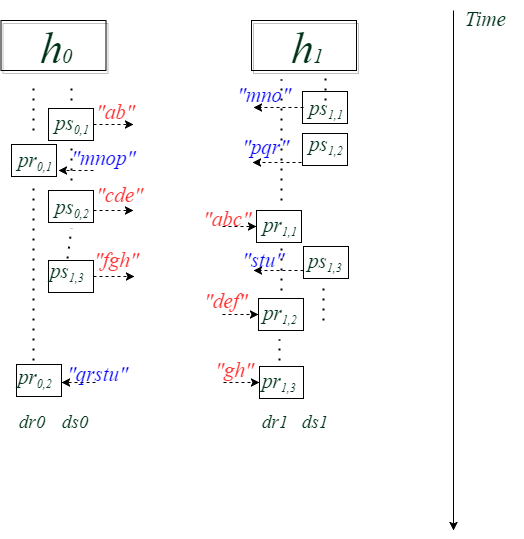
\includegraphics[scale=0.55]{Figures/reliableexample}}
\caption{Example of Reliable Communication}
\label{reliableexample}
\end{figure}

In this example, the payloads of the packages are:

$pl(pks_01)=``ab"$, $ pl(pks_02)=``cde"$, $pl(pks_03)=``fgh"$;

$pl(pkr_11)=``abc"$, $pl(pkr_12)=``def"$, $pl(pkr_13)=``gh"$ .

and 

$pl(pks_11)=``mno"$, $pl(pks_12)=``pqr"$, $pl(pks_13)=``stu"$;

$pl(pkr_01)=``mnop"$, $pl(pkr_02)=``qrstu"$. 

on the other direction. Their properties:

$pl(pks_01) \cdot pl(pks_02) \cdot pl(pks_03) = pl(pkr_11) \cdot pl(pkr_12) \cdot pl(pkr_13) = ``abcdefgh"$ and 

$pl(pks_11) \cdot pl(pks_12) \cdot pl(pks_13) = pl(pkr_01) \cdot pl(pkr_02) = ``mnopqrstu"$. 

satisfy the content preservation. 

The relative time relationship of the packages are: 

$time(pks_01) < time(pks_02) < time(pkr_11)< time(pks_03) < time(pkr_12) < time(pkr_13) $;

$time(pks_11) < time(pks_12) < time(pkr_01)< time(pks_13) < time(pkr_02)$. 

The fact that
 
$pl(pkr_01) = ``mnop"$ is the prefix of $pl(pks_11) \cdot  pl(pks_12) = ``mnopqr"$,

$pl(pkr_01) \cdot pl(pkr_02)=``mnopqrstu"$ is the prefix of(is this case identical to ) $pl(pks_11) \cdot pl(pks_12) \cdot pl(pks_13) = ``mnopqrstu" $,  

$pl(pkr_11)=``abc"$ is the prefix of $pl(pks_01 \cdot pl(pks_02) = "abcde"$,  

$pl(pkr_11) \cdot pl(pkr_12)= ``abcdef"$ and  $pl(pkr_11) \cdot pl(pkr_12) \cdot pl(pkr_13) = ``abcdefgh"$ are  the prefix of  $pl(pks_01) \cdot pl(pks_02) \cdot pl(pks_03)= ``abcdefgh"$

satisfy the timing preservation. 


Figure\ref{unreliableexample} is an example of the unreliable communication. 

\begin{figure}[H]
\centerline{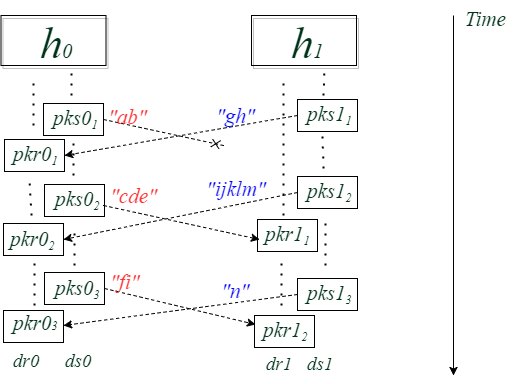
\includegraphics[scale=0.55]{Figures/unreliableexample}}
\caption{Example of Unreliable Communication}
\label{unreliableexample}
\end{figure}

In this example:

$pkr_11 = pks_02=``cde"$, $time(pkr_11) > time(pks_02)$; 

$pkr_12 = pks_02=``cde"$, $time(pkr_12) > time(pks_02)$; 

$pkr_13 = pks_03=``fi"$, $time(pkr_13) > time(pks_03)$;

$pkr_01 = pks_11=``gh"$, $time(pkr_01) > time(pks_11)$;

$pkr_02 = pks_12=``ijklm"$, $time(pkr_02) > time(pks_12)$;

$pkr_03 = pks_13=``n"$, $time(pkr_03) > time(pks_13)$.

All of these satisfy the content preservation and timing preservation of the unreliable communication.


	\startchapter{Prototype}
\label{chapter:newsol}

In this section we discuss the design of the prototype of dual-trace analysis. This prototype consist of three main components: user interface for defining the communication type, algorithm of locating the communication events in the dual-trace, user interface and strategy to navigate the located events to the sender and receiver traces. We provide the background information of the design of each component as well as their detail design in each corresponding subsection.
\subsection{User Defined Communication Type}
In our design, we don't specify any predefined communication type but give the user ability to do that. By the user interface implemented, the user can defined their own communication type. This give the flexibility to the user to define what they are looking for. Each communication type consist of 4 system function calls. They are channel create/open in sender and receiver sides, sender's send message function and receiver's receive message function. By indicating the channel create/open functions in both sender and receiver sides, the tool can acquire the channel's identifiers. Later on the tool can match the send and received messages within a specific channel. The send and receive functions are used to located the event happened in the traces. The messages sent and received are reconstructed from the memory state when the send and receive functions are called and returned. The detail of the match algorithm will be discuss later.

\subsubsection{Function Calls in the Traces}
The called functions' name can be inspected  by  search of the symbolic name in the executable binary or any DLLs which used by the program at the time when it is traced. This functionality exists in the current Atlantis. By importing the DLLs and execution  executable binary, Atlantis can list all called functions for the users in the Functions view. From this list, users can chose the interested functions and generate their interested communication type. In Figure\ref{functionsview} there is  an action item "Add to Communication type" in the right click menu of the function entry. Figure \ref{dialog} shows the dialogue for entering the information for the adding function. As this figure shows, users can get the existing communication type list in the drop down menu. They can choose to add the current function to an exist communication type or they can add it to a new communication type by entering a new name. For the channel create/open function, the register holding the address of channel's name as input and the register holding the handle identification of the channel as output are required. For the send/receive function, the register holding the address of the send/receiver buffer, the register holding the length of the sending/receiving message and the register holding the channel's identification are required. As there are 4 functions for each communication type users have to repeat this add function to communication type action for 4 times to generate one communication type.

\begin{figure}[h]
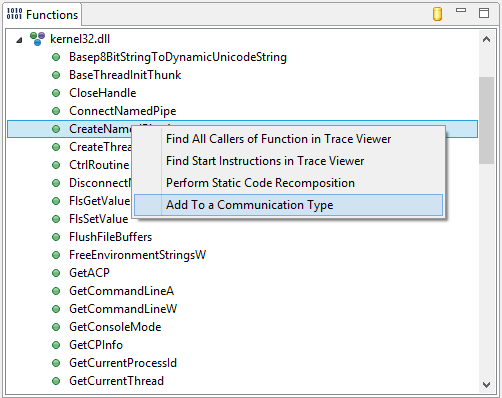
\includegraphics{Figures/functionsview}
 \caption{Add function to a Communication type from Functions View}
\label{functionsview}
\end{figure}

\begin{figure}[h]
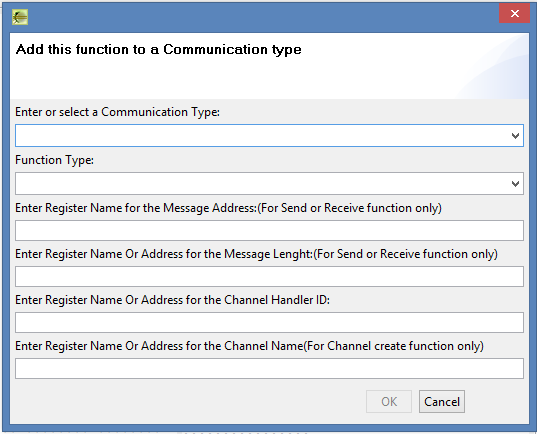
\includegraphics{Figures/dialog}
 \caption{Dialog to input information for a function adding to a communication type}
\label{dialog}
\end{figure}

\subsubsection{Communication Type Data Structure}
The defined communication type will be stored in a xml file. The list below shows the data structure of one communication type. 
\begin{lstlisting}
<messageTypesData>
    <parentFolder>.tmp</parentFolder>
    <messageTypes>
        <messageType>
            <name>namedPipe_clientsend</name>
            <sendFunction>
                <associatedFileName>Client</associatedFileName>
                <name>WriteFile</name>
                <messageAddress>RDX</messageAddress>
                <messageLengthAddress>R8</messageLengthAddress>
                <channelIdReg>RCX</channelIdReg>
            </sendFunction>
            <receiveFunction>
                <associatedFileName>Server</associatedFileName>
                <name>ReadFile</name>
                <messageAddress>RDX</messageAddress>
                <messageLengthAddress>R8</messageLengthAddress>
                <channelIdReg>RCX</channelIdReg>
            </receiveFunction>
            <sendChannelCreateFunction>
                <associatedFileName>Client</associatedFileName>
                <name>CreateFileA</name>
                <channelIdReg>RAX</channelIdReg>
                <channelNameAddress>RCX</channelNameAddress>
            </sendChannelCreateFunction>
            <receiveChannelCreateFunction>
                <associatedFileName>Server</associatedFileName>
                <name>CreateNamedPipeA</name>
                <channelIdReg>RAX</channelIdReg>
                <channelNameAddress>RCX</channelNameAddress>
            </receiveChannelCreateFunction>
        </messageType>
    </messageTypes>
</messageTypesData>
\end{lstlisting}


\subsubsection{Communication Type View}
A new view named Communication Types view is for the user defined communication types. All user defined communication type are stored in the .xml file and listed in communication type view when it's opened as shown in Figure \ref{CommunicationTypeview}. User can change the name of a communication type, remove an existing communication type or searching of the match message occurrences of selected communication type by selecting action item in the right click menu of an communication type entry. The matched messages are listed in the result window of the view. By clicking the entry of the search  result, user can navigate to it's sender or receiver's corresponding instruction line as shown in Figure\ref{searchresult}. Message content in the memory view will be shown as well.


\begin{figure}[h]
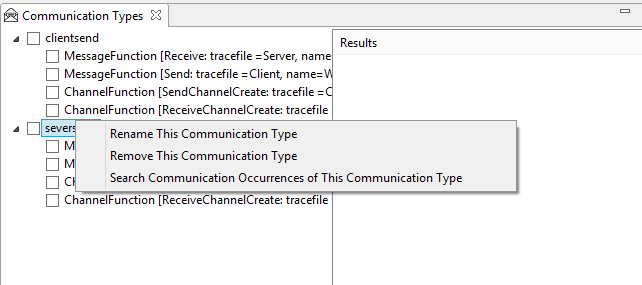
\includegraphics[scale=.9]{Figures/CommunicationTypeview}
 \caption{New View: Communication Type View}
\label{CommunicationTypeview}
\end{figure}

\begin{figure}[h]
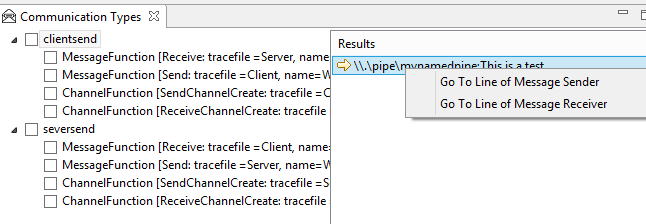
\includegraphics[scale=.9]{Figures/searchresult}
 \caption{Right Click menu to navigate to send and receive event in the traces}
\label{searchresult}
\end{figure}

\subsection{Communication Event Searching}
The communication event consists of the send message event in the sender side and receive message event in the receiver side. The communication event searching algorithm can be divided into three main steps: 1. search all channel create/open event in the sender and receiver side, save the handle id and corresponding channel name. 2. Search all message send and receive event in sender and receiver sides. 3. Matching the send/receive messages pair based on the channel names and message contents.
\subsubsection{Record opened Channel}
In this step the algorithm is supposed to search all the open channel both in the sender and receiver side. The found created channels are recorded in a map. The key of the map is the handler id of the channel and the value is the channel name. A channel in the sender and receiver sides will have different handler id but same channel name.
\subsubsection{Search send and receive Message}
All send message and receive message function calls will be found out in the trace. When a send function hit, the memory state of the hit instruction line will be reconstructed, and the message content can be get from the memory with the send message buffer address. When a receive function hit, the return line of that function is needed for getting the message content. The memory state of the function return line is reconstructed and the message content can be get  from the reconstructed memory state with the receive message buffer address.
\subsubsection{Matching the send/receive messages pair}
After the created channel and send/receive message are found out in the sender and receiver side, a matching algorithm is used to match the send/receive message pairs.
\subsubsection{Matching Event Data Structure}
The matching event is stored in cache when the tool is running. Only the most recent search result is cached currently. If users need the previous result, they need to apply the search again. The matching Event consist of two sub-events, one is message send event while the other is message receive event. Both of these two sub-events are object of BfvFileMessageMatch. BfvFileMessageMatch is an Java class extends org.eclipse.search.internal.ui.text.FileMatch. FileMatch class containing the information needed to navigate to the trace file editor. In order to show the corresponding send/receive message in the memory view, the target memory address storing the message content is set in BfvFileMessageMatch. Two more elements: message and channel name are also set in BfvFileMessageMatch which are listed in the search result. 

\subsection{Matching Event Visualization and Navigation}
The right click menu of an entry in the search result list has two action items: Go To Line of Message Sender and Go To Line of Message Receiver. Both of the action items allow users to navigate to the trace Instruction view. When the user click on these items, it will navigate to the corresponding trace sender or receiver trace instruction view.  Meanwhile the memory view jumps to the target address of the message buffer, and the memory state is reconstructed so that the message content in that buffer will be shown in the memory view.


	\startchapter{Experiments}
\label{chapter:Exp}

The case we used to test this prototype contains one named pipe synchronous channel between a server and a client. Client send a message to the server and server reply another message to the client. 
\subsection{Test and Verification Design}
The test cases are designed to find all the messages from client to server and all the messages from server to client. Two end to end test cases are designed for both scenarios. 

In each test case, there are three test steps: 1. define the communication type by adding channel creating functions and message send/receive functions of server and client sides. 2. search for the events of  the defined communication type. 3. for the occurrence of the events, navigate to the trace instruction and memory view.

Verification points are specified for each step as: 1. verify the communication types with their functions are listed in the communication view. 2. verify the message events in the dual-trace can be found and listed in the search result view. 3. verify the navigation from the result entry to the instruction view of sender trace and receiver trace.
\subsection{Result}
We used the dual-trace provided by DRDC and follow the experiment and verification design to conduct this test. Figure\ref{addcomtyperesult} shows that the user defined clientsend and serversend communication types are shown in the communication type view as well as the functions consist of the communication types. Figure\ref{occclientresult} shows the search result of clientsend communication type, while Figure\ref{occclientresult} shows the search result of the serversend communication type. By clicking the Go To Line of Message Sender and Go To Line of Message Receiver action items, instruction view and memory view updated correctly. Figure\ref{send} shows the server was sending out a message: This is an answer. 


\begin{figure}[H]
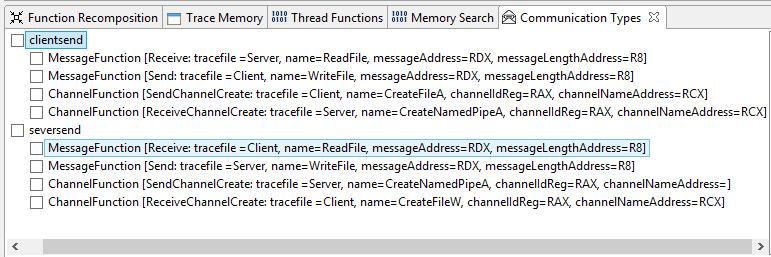
\includegraphics[scale=.72]{Figures/addcomtyperesult}
 \caption{Defined clientsend and serversend communication types in Communication View}
\label{addcomtyperesult}
\end{figure}

\begin{figure}[H]
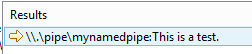
\includegraphics{Figures/occclientresult}
 \caption{the search result of clientsend communication type}
\label{occclientresult}
\end{figure}


\begin{figure}[H]
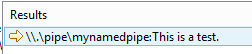
\includegraphics{Figures/occclientresult}
 \caption{the search result of the serversend communication type}
\label{occclientresult}
\end{figure}

\begin{figure}[H]
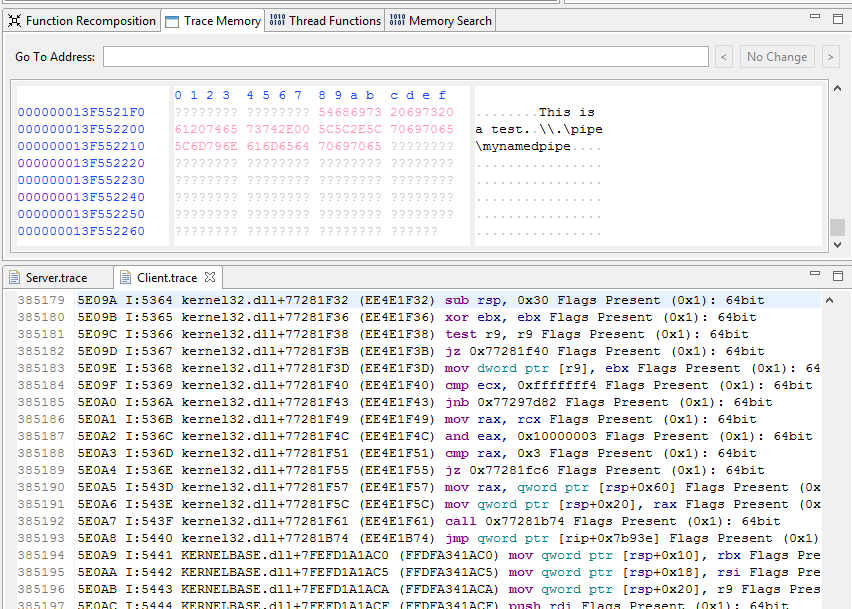
\includegraphics[scale=.66]{Figures/send}
 \caption{instruction view and memory view updated correctly}
\label{send}
\end{figure}

	\externaldocument{../appendix/chapter_app}
\externaldocument{../4/chapter_algorithm}
\externaldocument{../3/chapter_modeling}
\startchapter{Proof of Concept}
\label{chapter:Exp}
In this section, I present two experiments I ran for the proof of concept of the communication analysis though execution traces.

These experiments aimed to test the communication model and the communication identification approach. They also verify the design of the some algorithms, for their correctness.  

User case study is not included in this thesis and can be the future work. The feature prototype implementation is not evaluated and can be part of the user case study. But I used the implemented feature on Atlantis to conduct the experiments.

I first present the design of the experiments and their result. And then, I discuss the result of the experiments.  

\section{Experiments}
In this section, I describe the design of the experiments. Two experiments are conducted in this research. All test programs in these two experiments were written in C++ and the source code can be found in Appendix \ref{expcode}. Our research partner DRDC executed the programs in their environment and provided the captured traces, the used .dll files and the source code of the programs for the experiments.

Results are provided for each experiment. Both of the conducted experiments were about named pipe communication method. The following two subsections provides the details of the experiments and their result.

\subsection{Experiment 1}
In the first experiment, two programs communicated with each other through a synchronous Named pipe channel. One of the programs acted as the Named pipe server while the other as the client. Figure \ref{exp1} is the sequence diagram of the interaction between the server and client. Traces were captured while these two program were running and interacting. The two captured traces were analysed as dual\_trace $exp1$ in this experiment. I used the implemented features in Atlantis to analyse this dual\_trace. I ran the ``Stream identification" and ``Communication identification" operations for this dual\_trace. The streams and communication are showed in Figure\ref{result1}.

\begin{figure}[H]
\centerline{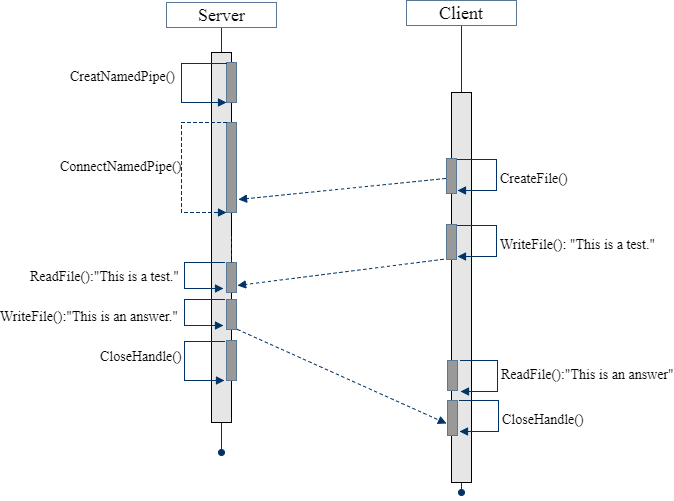
\includegraphics[scale=0.7]{Figures/exp1}}
 \caption{Sequence Diagram of Experiment 1}
\label{exp1}
\end{figure}

\begin{figure}[H]
\centerline{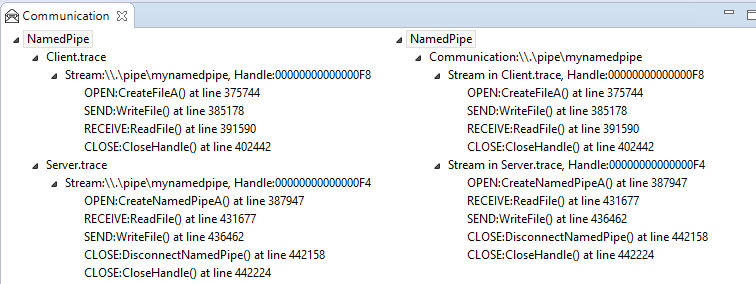
\includegraphics[scale=0.65]{Figures/result1}}
 \caption{Identification result of $exp1$}
\label{result1}
\end{figure}

\subsection{Experiment 2}
In the second experiment, one program was running as the Named pipe server. In this server program, four named pipes were created and can be connected by up to four client at a time. Two other programs as the Named pipe clients connected to this server. Those two clients (client 1 and client 2) used the identical program but run in sequence. Figure \ref{exp2} is the sequence diagram of the interaction among the server and clients. The function calls' sequence is only a possible combination from analyzing the source code. The real happening sequence can varies. Traces were captured at the time when these three programs were running and interacting. One trace for each program. The three traces are analysed as two dual\_traces, $exp2.1$ and $exp2.2$. $exp2.1$ consists of traces of server and client 1 and $exp2.2$ consists of traces of server and client 2. I ran the ``Stream identification" and ``Communication identification" operations for these two dual\_trace. The identified streams and communications are shown in Figure \ref{result21} and Figure \ref{result22}.

\begin{figure}[H]
\centerline{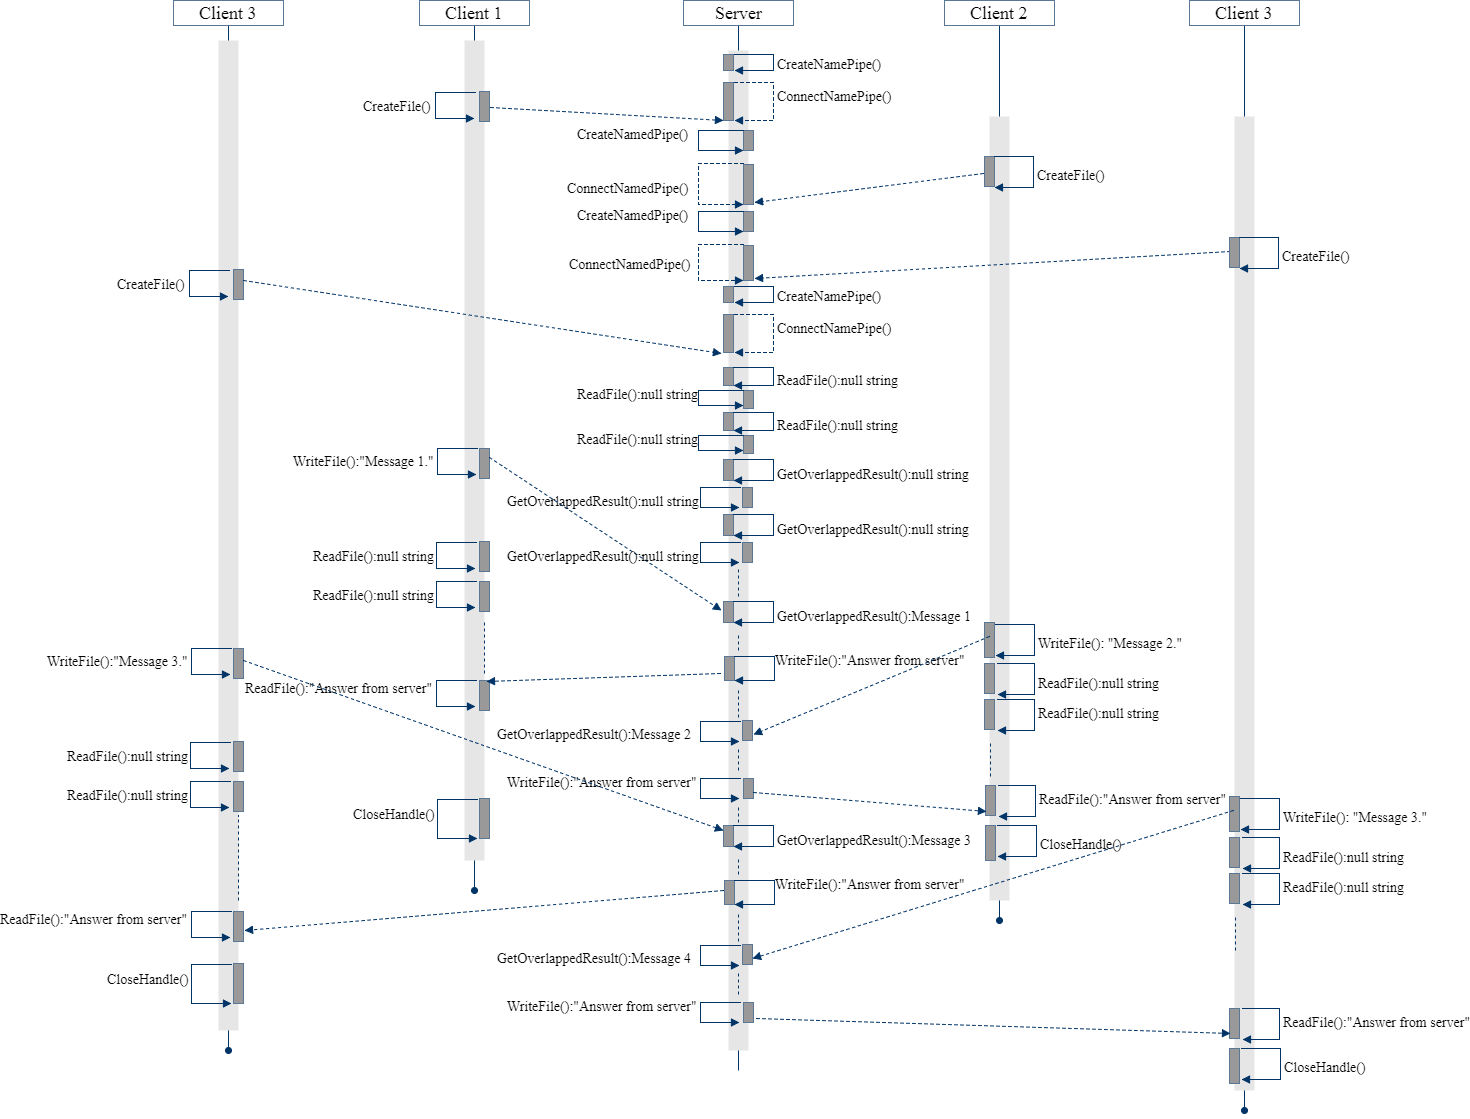
\includegraphics[scale=0.6]{Figures/exp2}}
 \caption{Sequence Diagram of Experiment 2}
\label{exp2}
\end{figure}

\begin{figure}[H]
\centerline{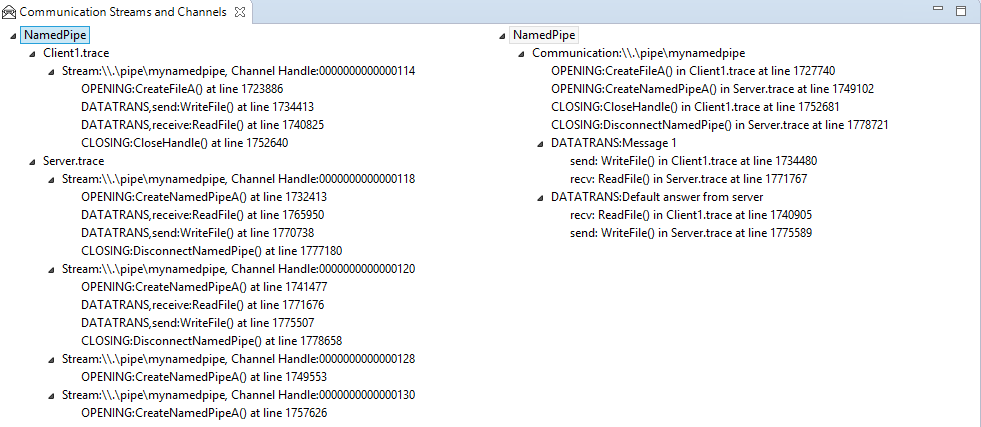
\includegraphics[scale=0.55]{Figures/result21}}
 \caption{Identification result of $exp2.1$}
\label{result21}
\end{figure}

\begin{figure}[H]
\centerline{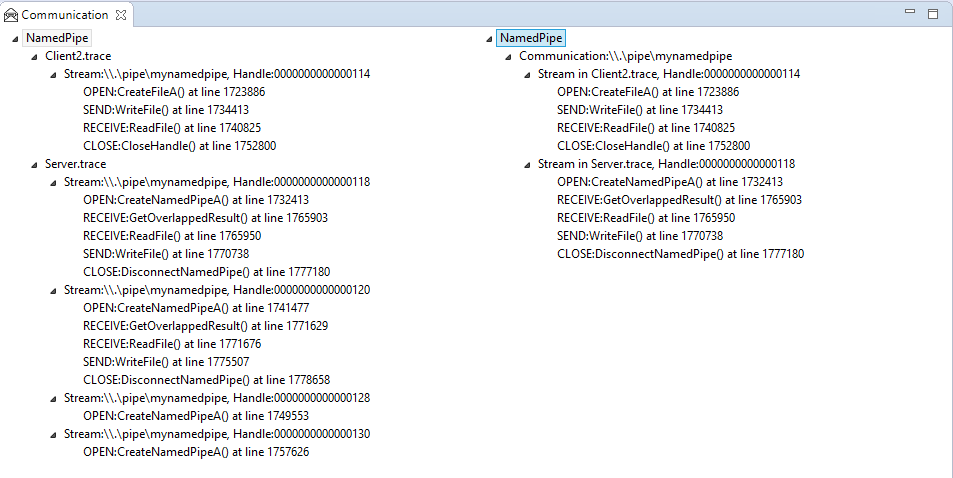
\includegraphics[scale=0.55]{Figures/result22}}
 \caption{Identification result of $exp2.1$}
\label{result22}
\end{figure}


\section{Discussion}
In the result of $exp1$, there are one stream extracted in client trace and one in server trace, and these two streams are matched into a communication of this dual\_trace. This identification result represents the actual communication happen between the named pipe server and client.
In the result of $exp2.1$ and $exp2.2$, there are one stream in each of the client traces and four in the server trace respectively. The streams are further matched and verified and eventually one communication is identified for each dual\_trace. The result aligns to the sequence diagram in Figure\ref{exp2}.


   





	\startchapter{Conclusions and Future Work}
\label{concl}
In this thesis, I present the approach of communication analysis through assembly level execution traces. I first defined the communication model. This abstract model depicts the outline of a communication between two running program, which gives the ground rule for the communication analysis. Then I depicted the general definition of the dual\_trace, the definition indicate that all traces comply to this definition can be used to conducted the communication analysis.

I also developed the essential algorithms for the communication identification. The high level algorithm is generalizable for all communication methods' identification while  the event stream extraction and matching algorithm are distinct for each communication method according to their channel open and data transfer mechanisms. However, the developed algorithms provides clear and referable examples to develop your own algorithm for communication methods which are not discussed in this thesis.

On top of the existing execution trace analysis environment Atlantis, I implemented the communication identification features. This feature provides the users a way to extend their concerned communication methods through the configuration file. The user interface allows the users to conduct the communication and stream identification from the dual\_traces and navigate back from the identified result to the views of the trace in Atlantis. This feature prototype is a novel feature for conducting multiple trace analysis for reverse engineering at the time when this thesis was written. The experiments conducted in this work preliminary proves the usability of the model and the algorithms. 

This thesis illustrates the novel idea and approach for dynamic program analysis which considerate the interaction of two programs. This idea is valuable due to the fact that programs or malware in the real world work collaboratively. The analysis of the communication and interaction of the programs provide more reliable information for vulnerability detection and program analysis.

Future work can be divided in two directions. One is extending the model to be more generalize for all kinds of interaction but not only the message transferring communications while the other is conducting user studies of the communication analysis approach and the feature design to get a more concrete result of their usefulness.


	\appendix
	\begin{appendices}	
\chapter{Microsoft x64 Calling Convention for C/C++}\label{convention}
\begin{itemize}  
\item RCX, RDX, R8, R9 are used for integer and pointer arguments in that order left to right.
\item XMM0, 1, 2, and 3 are used for floating point arguments.
\item Additional arguments are pushed on the stack left to right. \ldots 
\item Parameters less than 64 bits long are not zero extended; the high bits contain garbage.
\item Integer return values (similar to x86) are returned in RAX if 64 bits or less.
\item Floating point return values are returned in XMM0.
\item Larger return values (structs) have space allocated on the stack by the caller, and RCX then contains a pointer to the return space when the callee is called. Register usage for integer parameters is then pushed one to the right. RAX returns this address to the caller.
\end{itemize}

\chapter{Function Descriptor Configuration file Example}\label{funcset}
\lstinputlisting[caption= communicationMethods.json]{./sourcecode/communicationMethods.json}

\chapter{Code of the Parallel Editors}\label{paralleleditor}
Two essential pieces of code are listed for the parallel editor. One is for splitting the editor area for two editors while the other is to get the active parallel editors later on  for dual\_trace analysis.
\section{The Editor Area Split Handler}
\begin{lstlisting}[caption= code in OpenDualEditorsHandler.java]
public class OpenDualEditorsHandler extends AbstractHandler {
	EModelService ms;
	EPartService ps;
	WorkbenchPage page;

	  
    public Object execute(ExecutionEvent event) throws ExecutionException {
		IEditorPart editorPart = HandlerUtil.getActiveEditor(event);
		if (editorPart == null) {
			Throwable throwable = new Throwable("No active editor");
			BigFileApplication.showErrorDialog("No active editor", "Please open one file first", throwable);
			return null;
		}

		MPart container = (MPart) editorPart.getSite().getService(MPart.class);
		MElementContainer m = container.getParent();
		if (m instanceof PartSashContainerImpl) {
			Throwable throwable = new Throwable("The active file is already opened in one of the parallel editors");
			BigFileApplication.showErrorDialog("TThe active file is already opened in one of the parallel editors",
					"The active file is already opened in one of the parallel editors", throwable);
			return null;
		}
		IFile file = getPathOfSelectedFile(event);

		IEditorDescriptor desc = PlatformUI.getWorkbench().getEditorRegistry().getDefaultEditor(file.getName());
		try {
			IFileUtils fileUtil = RegistryUtils.getFileUtils();
			File f = BfvFileUtils.convertFileIFile(file);
			f = fileUtil.convertFileToBlankFile(f);
			IFile convertedFile = ResourcesPlugin.getWorkspace().getRoot().getFileForLocation(Path.fromOSString(f.getAbsolutePath()));
			convertedFile.getProject().refreshLocal(IResource.DEPTH_INFINITE, null);
			if (!convertedFile.exists()) {
				createEmptyFile(convertedFile);
			}

			IEditorPart containerEditor = HandlerUtil.getActiveEditorChecked(event);
			IWorkbenchWindow window = HandlerUtil.getActiveWorkbenchWindowChecked(event);
			ms = window.getService(EModelService.class);
			ps = window.getService(EPartService.class);
			page = (WorkbenchPage) window.getActivePage();
			IEditorPart editorToInsert = page.openEditor(new FileEditorInput(convertedFile), desc.getId());
			splitEditor(0.5f, 3, editorToInsert, containerEditor, new FileEditorInput(convertedFile));
			window.getShell().layout(true, true);
			

		} catch (CoreException e) {
			e.printStackTrace();
		}

		return null;
	}

    private void createEmptyFile(IFile file) {
		byte[] emptyBytes = "".getBytes();
		InputStream source = new ByteArrayInputStream(emptyBytes);
		try {
			createParentFolders(file);
			if(!file.exists()){
				file.create(source, false, null);
			}
		} catch (CoreException e) {
			e.printStackTrace();
		}finally{
			try {
				source.close();
			} catch (IOException e) {
				// Don't care
			}
		}
	}

	private void splitEditor(float ratio, int where, IEditorPart editorToInsert, IEditorPart containerEditor,
			FileEditorInput newEditorInput) {
		MPart container = (MPart) containerEditor.getSite().getService(MPart.class);
		if (container == null) {
			return;
		}

		MPart toInsert = (MPart) editorToInsert.getSite().getService(MPart.class);
		if (toInsert == null) {
			return;
		}

		MPartStack stackContainer = getStackFor(container);
		MElementContainer<MUIElement> parent = container.getParent();
		int index = parent.getChildren().indexOf(container);
		MStackElement stackSelElement = stackContainer.getChildren().get(index);

		MPartSashContainer psc = ms.createModelElement(MPartSashContainer.class);
		psc.setHorizontal(true);
		psc.getChildren().add((MPartSashContainerElement) stackSelElement);
		psc.getChildren().add(toInsert);
		psc.setSelectedElement((MPartSashContainerElement) stackSelElement);

		MCompositePart compPart = ms.createModelElement(MCompositePart.class);
		compPart.getTags().add(EPartService.REMOVE_ON_HIDE_TAG);
		compPart.setCloseable(true);
		compPart.getChildren().add(psc);
		compPart.setSelectedElement(psc);
		compPart.setLabel("dual-trace:" + containerEditor.getTitle() + " and " + editorToInsert.getTitle());

		parent.getChildren().add(index, compPart);
		ps.activate(compPart);

	}

	private MPartStack getStackFor(MPart part) {
		MUIElement presentationElement = part.getCurSharedRef() == null ? part : part.getCurSharedRef();
		MUIElement parent = presentationElement.getParent();
		while (parent != null && !(parent instanceof MPartStack))
			parent = parent.getParent();

		return (MPartStack) parent;
	}


	private IFile getPathOfSelectedFile(ExecutionEvent event) {
		IWorkbenchWindow window = PlatformUI.getWorkbench().getActiveWorkbenchWindow();
		if (window != null) {
			window = HandlerUtil.getActiveWorkbenchWindow(event);
			IStructuredSelection selection = (IStructuredSelection) window.getSelectionService().getSelection();
			Object firstElement = selection.getFirstElement();
			if (firstElement instanceof IFile) {
				return (IFile) firstElement;
			}
			if (firstElement instanceof IFolder) {
				IFolder folder = (IFolder) firstElement;
				AtlantisBinaryFormat binaryFormat = new AtlantisBinaryFormat(
						folder.getRawLocation().makeAbsolute().toFile());
				// arbitrary, just any file in the binary set is needed
				return AtlantisFileUtils.convertFileIFile(binaryFormat.getExecVtableFile());
			}
		}
		return null;
	}
}
\end{lstlisting}

\section{Get the Active Parallel Editors}
\begin{lstlisting}[caption= code for getting parallel editors ]
IEditorPart editorPart = PlatformUI.getWorkbench().getActiveWorkbenchWindow().getActivePage().getActiveEditor();
		MPart container = (MPart) editorPart.getSite().getService(MPart.class);
		MElementContainer m = container.getParent();
		if (!(m instanceof PartSashContainerImpl)) {
			Throwable throwable = new Throwable("This is not a dual-trace");
			BigFileApplication.showErrorDialog("This is not a dual-trace!", "Open a dual-trace First", throwable);
			return;
		}

		MPart editorPart1 = (MPart) m.getChildren().get(0);
		MPart editorPart2 = (MPart) m.getChildren().get(1);
\end{lstlisting}

\chapter{Code of the Programs in the Experiments}\label{expcode}
\section{Experiment 1}
The two interacting programs were Named pipe server and client. The first piece of code listed below is the code for the server's program while the second piece is for the client program.
\lstinputlisting[language=C++,caption= NamedPipeServer.cpp]{./sourcecode/experiment1/NamedPipeServer.cpp}
\lstinputlisting[language=C++,caption= NamedPipeClient.cpp]{./sourcecode/experiment1/NamedPipeClient.cpp}

\section{Experiment 2}
In the experiment 2, two clients run the same program in sequence to connect to the server with asynchronous Named pipe channel. The first piece of code listed below is the code for the server's program while the second piece is the test.bat is the script for running the experiment. The client  program's code is identical to experiment 1.
\lstinputlisting[language=C++,caption= NamedPipeServerOverlapped.cpp]{./sourcecode/experiment2/NamedPipeServerOverlapped.cpp}
\lstinputlisting[caption= test.bat]{./sourcecode/experiment2/test.bat}

\end{appendices}

% The style of bibliography exemplified here is the "plain",
% normally used in science theses. This is shown
% by the entry {plain} below. Substitute the
% appropriate bibliography style. See also the
% PDF file "InformationOnBibliographyStyles" in this
% directory for more choices.

% The Bibliography file is a BibTex file named
% UVicThesis.bib and called below

	\TOCadd{Bibliography}
	\bibliographystyle{plain}
	\bibliography{UvicThesis}

\end{document}
